\documentclass[serif,9pt]{beamer}
\usepackage{color,listings}
\usepackage{ragged2e}
\usepackage[spanish]{babel}
\usepackage{graphicx}

\definecolor{dkgreen}{rgb}{0,0.6,0}
\definecolor{gray}{rgb}{0.5,0.5,0.5}
\definecolor{mauve}{rgb}{0.58,0,0.82}
\definecolor{lgray}{rgb}{0.99,0.97,0.95}
\newcommand{\X}{\textbf{X}}
\newcommand{\Y}{\textbf{Y}}
\newcommand{\Z}{\textbf{Z}}
\newcommand{\G}{\textbf{G}}
\newcommand{\R}{\textbf{R}}
\newcommand{\V}{\textbf{V}}
\newcommand{\Q}{\textbf{Q}}
\newcommand{\h}{\textbf{H}}
\newcommand{\T}{\textbf{T}}

\def\E{\mathbb{E}}
\def\C{\mathbb{C}}
\def\N{\mathbb{N}}


\usetheme{Frankfurt}
%\usecolortheme{rose}
\usecolortheme{lily}
\usepackage{amsmath, multirow}
%\usepackage{color, amsmath, wrapfig, anysize, graphicx, hyperref, amsthm, fancyhdr, amssymb,geometry,amsfonts,float}

\newcommand{\ds}{\displaystyle}


\titlegraphic{
\includegraphics[width=4cm]{utfsm.eps}}%
   %\includegraphics[width=4cm]{fig/inria.eps}}

\begin{document}
\title[Una Arquitectura de Referencia para Web
Browsers]{Hacia una unificaci\'on de Conceptos de Seguridad} 
\author[Paulina Silva Ghio]{\textsc{Paulina Silva Ghio} \\ \medskip
\small{}
Departamento de Inform\'atica - UTFSM\\ \medskip
\url{pasilva@alumnos.inf.utfsm.cl}}
\institute[]{}
\date{24-11-2015.}

\begin{frame}[plain]
\titlepage
\end{frame}


\begin{frame}
\frametitle{Indice}
\tableofcontents
\end{frame} 


\section{Introducci\'on}
\subsection{Contexto}
\begin{frame}
\frametitle{Contexto}

	\begin{itemize}
		\item La guerra de los Navegadores: construir y parchar.
		\item El navegador web: herramienta de uso cotidiano.
		\item El usuario com\'un utiliza servicios.
		\item Distintos tipos, distintas implementaciones.
		\item Web 2.0 y 3.0: AJAX (Asynchronous Javascript and XML).
	\end{itemize}
\end{frame}


\begin{frame}
\frametitle{Browser en la Actualidad}
	\begin{figure}[h]
	    \centering
	    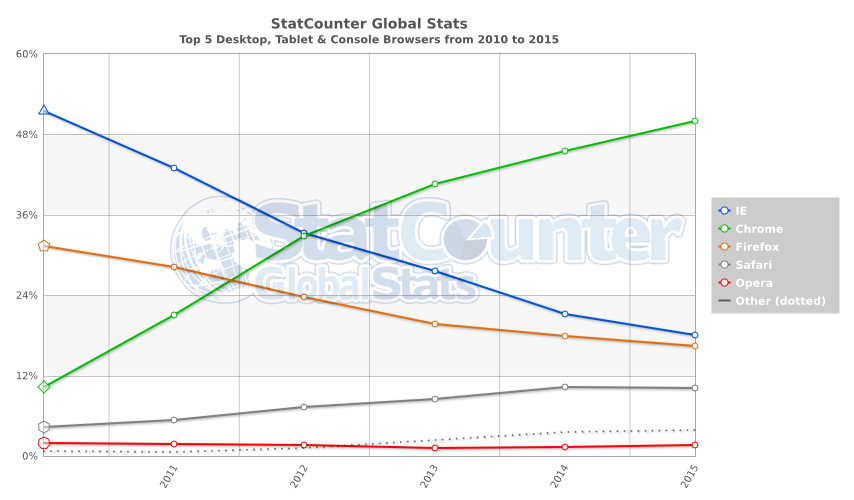
\includegraphics[width=1\textwidth]{figures/StatCounter-browser-ww-yearly-2010-2015.png}
	    \caption{Porcentaje de uso de Navegadores. Fuente: \cite{statBrow}}
	    \label{fig:UsageShare}
	\end{figure}
\end{frame}


\subsection{Seguridad...}
\begin{frame}
\frametitle{Seguridad...}
	\begin{block}{Desde la perspectiva de seguridad \cite{WhyteHarrison}:}
		\begin{itemize}		
			\item �Qu\'e realizan las universidades o la industria respecto a estas preocupaciones?
			\item Projectos de desarrollo de software, �cuanto se le dedica a la seguridad?
		\end{itemize}
	\end{block}
	\begin{block}{�Qu\'e conceptos de seguridad sabe en promedio un estudiante graduado de carrera relacionada a Computer Science?}
		\begin{itemize}
			\item �La gente es autodidacta? o �aprende por necesidad?
			\item �La malla curricular es suficiente?
			\item �La industria asegura que los sistemas a construir, sean seguros?
		\end{itemize}
	\end{block}
\end{frame}



\subsection{Desarrollo de Software y Seguridad}
\begin{frame}
\frametitle{Desarrollo de Software y Seguridad}
	\begin{itemize}
		\item �Qu\'e tanto se diferencian las preocupaciones del usuario com\'un y el desarrollador que crea los sistemas?
		\item �C\'omo desarrollar software seguro?
	\end{itemize}
	\begin{block}{Construcci\'on de Software Seguro...}
		\begin{itemize}
			\item Los que participan en la construcci\'on: deben entender los problemas de seguridad.
			\item No basta saber como est\'a construido.
			\item Considerar la Seguridad desde el inicio del Proyecto.
			\item Seguridad como una Propiedad Sist\'emica.
		\end{itemize}
	\end{block}
\end{frame}

\subsection{Motivaci�n para estudiar este tema}
\begin{frame}
	\frametitle{Motivaci�n}
	\begin{itemize}
		\item Nuevas formas de interactuar.
		\item Permite disminuir los costos de construir un programa Cliente (desde cero) para
el usuario del sistema.
		\item Seguridad implementada que los Web Browser es bastante buena.
		\item El browser es una herramienta indispensable.
	\end{itemize}

	\begin{block}{Las preocupaciones principales}
	\begin{itemize}
		\item Los sistemas, a los que un usuario hace referencia, son llamados desde un Web Browser.
		\item El stakeholder afectado: el usuario del Browser, el Host del usuario y hasta el Servicio externo usado.
		\item Falta de conocimientos de seguridad con respecto al Browser, podr�a afectar de forma directa el desarrollo de aplicaciones que lo utilizan.
	\end{itemize}

	\end{block}
\end{frame}

\subsection{Contribuciones}
\begin{frame}
	\frametitle{Contribuciones}
	\begin{block}{Objetivo General}
		\begin{itemize}
			\item Generar un cuerpo organizado de informaci�n sobre el Web Browser y su seguridad, de tal manera que se pueda sistematizar, organizar y clasificar el conocimiento adquirido en un documento, con formato semi-formal, tanto para Profesionales como Estudiantes del �rea Inform�tica que est�n insertos en el �rea de Desarrollo de Software.
		\end{itemize}
	\end{block}
\end{frame}

\begin{frame}
	\frametitle{Contribuciones}
	\begin{block}{Objetivos Espec�ficos}
		\begin{itemize}
			\item Comprender los conceptos relacionados al navegador web, sus componentes, interacciones o formas de comunicaci�n, amenazas y ataques a los que puede estar sometido, como tambi�n los mecanismos de defensa. Esto se realizar� a trav�s del desarrollo de un Estado del Arte sobre el Browser.
			\item Identificar actores, componentes, funciones, relaciones, requerimientos y restricciones del navegador, para lograr abstraer una Arquitectura de Referencia (AR) a partir de documentaci�n disponible en Internet, blogs de desarrolladores, papers e iniciar un peque�o cat�logo de Patrones de Mal Uso. Esto permitir� condensar el conocimiento obtenido en el punto anterior a trav�s de documentos semi-formales, lo que permitir� generar una gu�a para comunicar los conceptos relevantes que pudieran afectar la relaci�n existente entre un desarrollo de software y el navegador.
			\item Profundizar el conocimiento en ataques relacionados con m�todos de Ingenier�a Social
		\end{itemize}
	\end{block}
\end{frame}

\begin{frame}
	\frametitle{Arquitectura de Referencia (AR) y Patrones de Mal Uso}
	\begin{block}{AR}
		\begin{itemize}
			\item Metodolog�a base en Fernandez
			\item Capturar la esencia de la arquitectura a trav�s de una colecci�n de sistemas similares, por medio del reuso arquitect�nico
			\item Ayudar a los implementors o desarrolladores del software, a entender los trade-off cuando se dise�an nuevos sistemas
			\item Ayudar a los mantenedores de estos sistemas a entender el c�digo legacy usado.
			\item Comparar las diferencias en decisiones de dise�o y poder entender los cambios realizados a lo largo del Desarrollo de un sistema.
			\item Mirada hol�stica del Sistema.
		\end{itemize}
	\end{block}
	\begin{block}{Patrones del Mal Uso}
		\begin{itemize}
			\item Permitir�n ense�ar y comunicar las posibles formas en que tal sistema puede ser usado inapropiadamente.
		\end{itemize}
	\end{block}
\end{frame}



\bibliography{refTodas}
\bibliographystyle{IEEEtran}

\end{document}

